\section{Evaluation} \label{sec:evaluation}


In this section, we first use a case study (\S\ref{subsec:eva-casestudy}) given
in Figure \ref{fig:data-race} to show the complete workflow of \TheName. 
Next, we focus on evaluate \TheName{} with the four practical requirements
discussed in \S\ref{sec:introduction}.

We deploy \TheName on an Armv8 Juno r2 board equipped with 6 cores (2
Cortex-A72 cores and 4 Cortex-A53 cores) and 8GB RAM based on Linaro
deliverables Linux 5.4.50. We equip the Juno board with an SSD and allocate
256 MB circular buffers for ETM tracing. We use this as the default setting for
our experiment but also allowed developers to adjust it as required.

\subsection{Case Study} \label{subsec:eva-casestudy}


% Please add the following required packages to your document preamble:
% \usepackage{booktabs}
\begin{table*}[]
    \caption{Syscall Capturing Result for Figure~\ref{fig:data-race}}
    \label{study_case_flow}
    \centering
    \scalebox{0.62}{
    \begin{tabular}{@{}llll@{}}
        \toprule
        \textbf{Line} & \textbf{Thread 1}                           & \textbf{Thread 2}                                       & \textbf{Data Values}                                          \\ \midrule
        10              &                                             & bl 400910 \textless{}strlen@plt\textgreater{}           & total=0, len=0, buf=?                                          \\
        4              & bl 400960 \textless{}read@plt\textgreater{} &                                                         & read, fd=3, size=64, res=25,  data="1234567890123456789012345" \\
        12              &                                             & bl 400970 \textless{}strcpy@plt\textgreater{}           & total=0, len=875770417, buf=“123456789012345"                  \\
        4              & bl 400960 \textless{}read@plt\textgreater{} &                                                         & read, fd=4, size=64, res=6, data="123456"                      \\
        10              &                                             & bl 400910 \textless{}strlen@plt\textgreater{}           &                                                                \\
        12              &                                             & bl 400970 \textless{}strcpy@plt\textgreater{}           & total=875770423, len=6, buf="123456"                           \\
        14              &                                             & bl 400940 \textless{}\_\_assert\_fail@plt\textgreater{} &                                                                \\ \bottomrule
    \end{tabular}
    }
\end{table*}

To evaluate the functionality of \TheName, we test it with the program shown in
Figure \ref{fig:data-race}. As Table \ref{study_case_flow} illustrates, 
it is clear that Thread 2 checks the length of \texttt{big\_buf} (Line 10) before the first \texttt{read} (Line 4) in Thread 1. Since 
we capture the data of \texttt{read}, we know that the \texttt{big\_buf} contains 
a string with length 25. Therefore, the following \texttt{strcpy} (Line 12) incurs a buffer overflow, and the variable \texttt{len} (Line 7) 
is unexpectedly changed to \texttt{875770417}, which finally leads to the failure 
of the \texttt{assert} (Line 14). 

It is notable that the program does not crash immediately after the buffer 
overflow. In contrast, it executes normally for the second cycle. 
In addition, the normal execution of the second time overwrites the 
values (\texttt{buf} and \texttt{len}) involved in the buffer overflow, which 
may confuse developers without the assistance of \TheName.


\subsection{Completeness} \label{subsec:eva-flowaccuracy}

\begin{table}
    \caption{Buffer usage when file dumps}
    \centering
        \begin{tabular}{@{}lllll@{}}
            \toprule
            \multicolumn{1}{c}{\multirow{2}{*}{\textbf{Program}}} & \multirow{2}{*}{\textbf{\# dumping file}} & \multicolumn{3}{l}{\textbf{buffer usage}} \\
            \multicolumn{1}{c}{}                                  &                                           & Min.                & Max.               & Avg.               \\ \midrule
            nginx (5,000,000 requests)                                                  & 96                                        & 25                  & 360                & 183                \\
            large file read (40 GB)                                      & 79                                        & 39                  & 7,550               & 4,042               \\ \bottomrule
            \end{tabular}
    \label{table:Completeness}
\end{table}

% We evaluates the completeness of \TheName by following items:
Due to the implementation of the secondary buffer, the record may become incomplete because of not being transferred in time. We evaluate \TheName with two extreme scenarios: nginx with high concurrency and file reading with massive IO operations. As Table \ref{table:Completeness} shows,
 even in the worst case that 4,042 bytes, much less than 16 MB, is written to buffer before the secondary buffer dumping to file, \TheName ensures the completeness of the record.

\subsection{Effectiveness} \label{subsec:eva-Effectiveness}

\begin{table}
    \caption{Syscalls issued from bugs recorded by \TheName{}. N/A=bugid is not available, E=reconstructed bug, R=real-world bug, OV=order violaion, SAV=single variable atomicity violation, MAV=multi variables atomicity violation, DL=deadlock, SEQ=sequential bug (non-concurrency bug), LOC=line of code}
    \scalebox{1.0}{
        \begin{tabular}[]{@{}llll@{}}
            \toprule
            \textbf{Program-BugID-GroupType} & \textbf{bug type} & \textbf{LOC} & \textbf{Symptom}         \\
            \midrule
            shared\_counter-N/A-E            & SAV               & 45           & assertion failure        \\
            log\_proc\_sweep-N/A-E           & SAV               & 93           & segmentation fault       \\
            bank\_account-N/A-E              & SAV               & 95           & race condition fault     \\
            jdk1.4\_StringBuffer-N/A-E       & SAV               & 180          & assertion failure        \\
            circular\_list-N/A-E             & MAV               & 155          & race condition fault     \\
            mysql-169-E                      & MAV               & 120          & assertion failure        \\
            mutex\_lock-N/A-E                & DL                & 51           & deadlock                 \\
            SQLite-1672-R                    & DL                & 80K          & deadlock                 \\
            memcached-127-R                  & SAV               & 18K          & race condition fault     \\
            Python-35185-R                   & SAV               & 1256K        & race condition  fault    \\
            Python-31530-R                   & MAV               & 1256K        & segmentation fault       \\
            aget-N/A-R                       & MAV               & 2.5K         & assertion failure        \\
            pbzip2-N/A-R                     & OV                & 2K           & use-after-free           \\
            curl-965-R                       & SEQ               & 160K         & unhandled input pattern  \\
            cppcheck-2782-R                  & SEQ               & 120K         & unhandled input pattern  \\
            cppcheck-3238-R                  & SEQ               & 138K         & NULL pointer dereference \\
            \bottomrule
        \end{tabular}}
    \label{table:bug benchmarks}
\end{table}


We show how effectively \TheName is for diagnosing the root cause of bugs. As
listed in Table \ref{table:bug benchmarks}, we use 16 commonly C/C++ buggy
programs
\cite{cui2018rept,kasikci_lazy_2017,yu2009case,yu2012maple,kasikci2015failure, liang2020ript}
to evaluate \TheName.
% We focus on picking open-source software bugs for
% reproducibility in the ARM platform
We divide these bugs into two groups, i.e., Group E and Group R.
Group E contains 7 bugs reconstructed from
applications \cite{yu2009case,yu2012maple}, and Group R includes 9 bugs in
real-world applications
\cite{cui2018rept,kasikci_lazy_2017, kasikci2015failure, liang2020ript}.
There are 13 concurrency bugs, of which 6 are single variable atomicity
violation (SAV), 4 are multi variables atomicity violation (MAV), 2 are deadlock
(DL), and 1 is order violation (OV). There are also 3 non-concurrency bugs.
These bugs are collected from a diverse set of real-world systems (e.g., Python,
Memcached, SQLite, and Aget) and wide symptoms (e.g., NULL pointer dereference,
use-after-free, and race).



% The main limitation that restricts us to evaluate \TheName on more
% bugs is that we need to base on open-source software to reproduce and estimate
% the accuracy of bugs analysis, but most of the software reported bugs are
% difficult to install on ARM.

% In this section, we evaluate the effectiveness of \TheName by comparing our root
% cause results from Root Cause Detector with the bug fix report of the
% benchmarks we evaluated. 
% Note that, since our Root Cause Detector focus on
% working for automatic diagnosis of concurrency bugs, we obtain automatic
% analysis results about the root cause on 13 concurrent bugs in total. 
We execute these programs separately in our system until the bug occurs
and then use \TheName to record. And then anaylyze the root cause of bugs.
% We receive the identified root 
% cause from \TheName and confirm that it is effective for root cause analysis 
% of all the 16 bugs.
 Specifically, we manually analyze the bug by record and compare the related patches 
of these bugs. The result indicates that the failure reports
generated by \TheName are exactly related to the root cause.

Out of those 16 bugs, we select one representative
example to further demonstrate the effectiveness of \TheName.


% \subsubsection{Pragmatistic} \label{subsec:eva-Effectiveness-reversedebugging}

% In this section, we show that \TheName can help developers debug non-concurrency
% bugs through multiple debug techniques based on reconstructed execution history.

\begin{table}[]
    \caption{\TheName output of Cppcheck-2782}
    \label{table: The root cause of cppcheck}
    \centering
    \begin{tabular}{@{}llll@{}}
        \toprule
        \textbf{PID} & \textbf{\Syscall{}} & \textbf{Parameters} & \textbf{Additional
            information}
        \\ \midrule 22571        & getcwd           &    -                 &
        path=/home/root/cppcheck
        \\
        22571        & newfstatat       & res=0               & -
        \\
        22571        & fstat            & res=0               & fd=1
        \\
        22571        & write            & res=29              & -
        \\
        22571        & openat           & res=3               & dir=-100,
        path=./fail.cpp
        \\
        22571        & read             & fd=3                & data="int
        main() \{ return0; \}
        \\
                     &                  &                     &
        \begin{tabular}[c]{@{}l@{}}\#asm \\   !while (val)   mov
            bx                \\ \#endasm"\end{tabular}                                                  \\
        22571        & close            & fd=3                & res=0
        \\ \bottomrule
    \end{tabular}
\end{table}

\textbf{Cppcheck-2782.} In this case, we use \TheName to record a
non-concurrency bug. We run the application with common C++ source code as its
input until it crashes. Table \ref{table: The root cause of cppcheck} shows
the \syscall{}s recorded by \TheName. The C++ source
code analyzed by Cppcheck which triggered the bug is loaded with the \syscall{}
\texttt{read}. We then find the source code is special for containing embedded
assembly code. According to the public bug report, the Cppcheck-2782 is known as
a bug caused by unhandled input pattern, for its disability in handling embedded
assembly code. \TheName can help developer correctly locate the bug and easily analyze the root
cause.

\subsection{Efficiency} \label{subsec:eva-Efficiency}

We show how efficiently \TheName can be used for bug analysis by first running
Unixbench 5.1.2 \cite{unixbench} to measure the performance impact on kernel
such as \syscall{}. We then run ApacheBench \cite{ApacheBench} with Nginx 1.20
\cite{nginx_1.20.0}, representing a popular server program to simulate a high load
scenario. We finally evaluate the runtime performance overhead of \TheName by running four real-world programs.

\subsubsection{Unixbench} \label{subsec:eva-Performance-Unixbench}

\begin{figure}
    \centering
    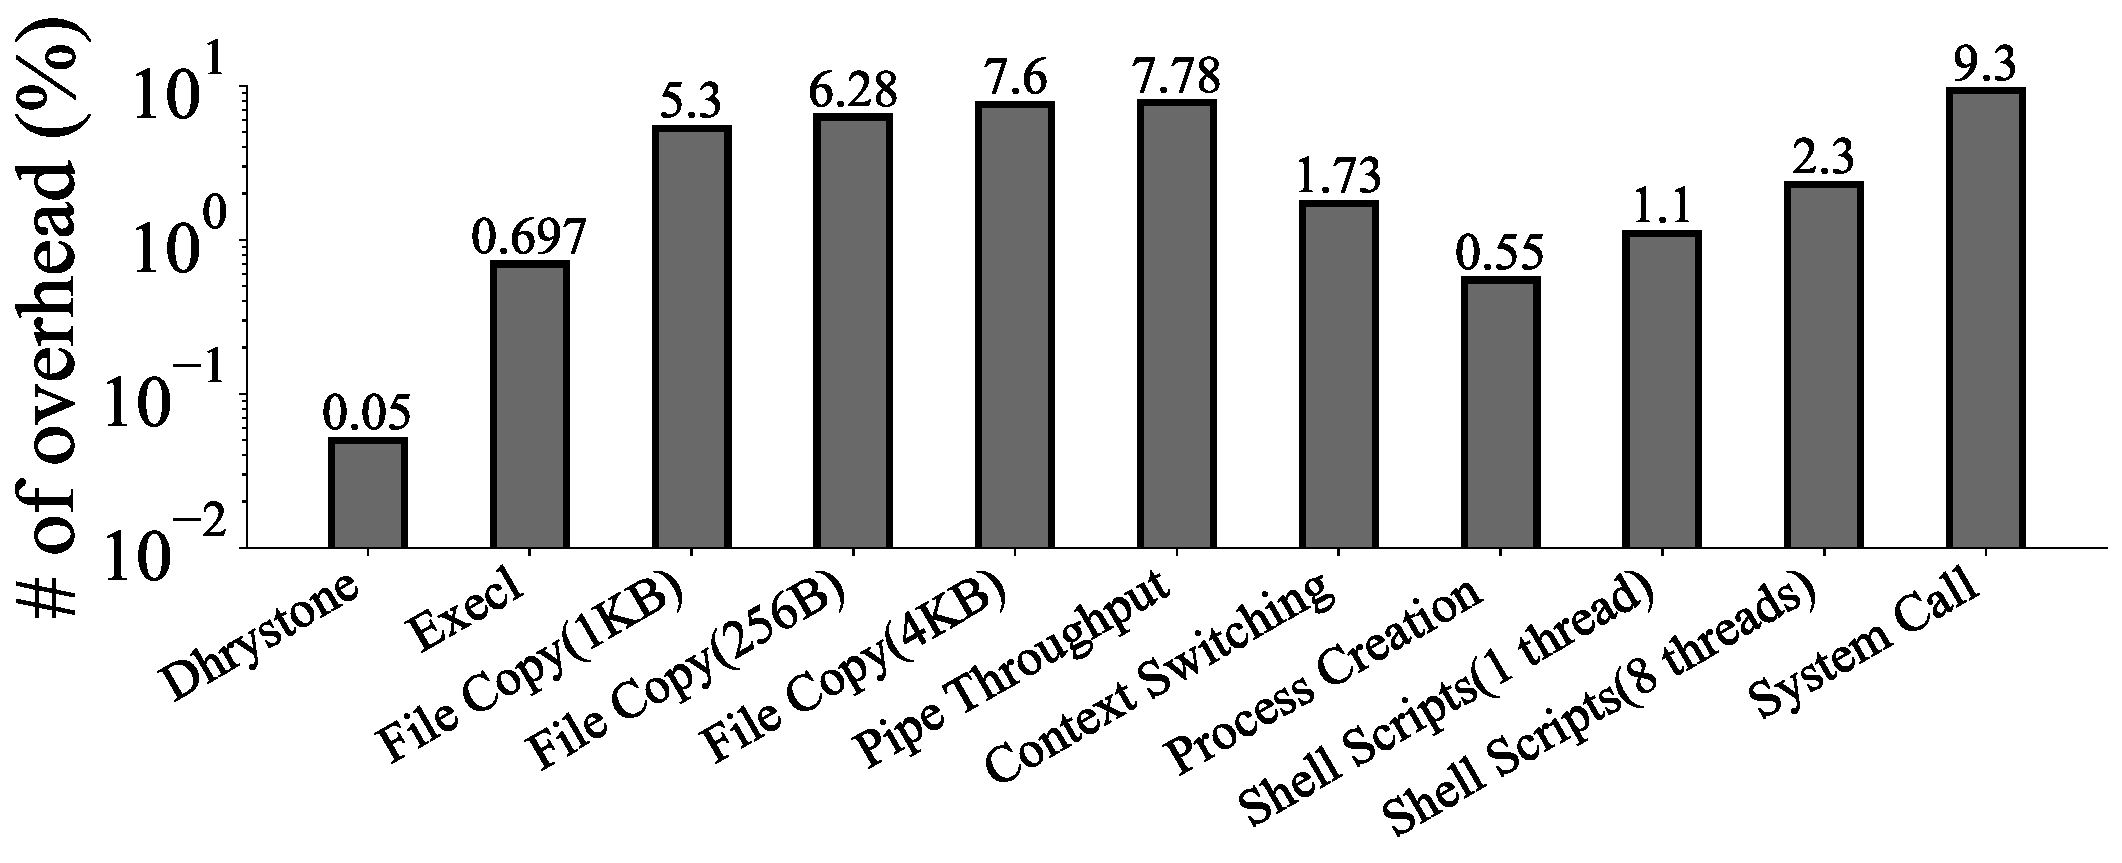
\includegraphics[width=0.9\textwidth]{figures/unixbenchoverheadbar.pdf}
    \caption{Performance overhead of UnixBench}
    \label{fig:Performance overhead of running UnixBench}
\end{figure}

We run UnixBench on Linux and show the performance results in Figure
\ref{fig:Performance overhead of running UnixBench}. For the tracing enabling,
the performance overhead is 3.88\% on average, and the highest performance
overhead is for System Call at 9.3\%. Specifically, there are three types of
benchmarks: File Copy, Pipe Throughput, and System Call that have higher
overhead. We believe that it is because these benchmarks have more frequent
\syscall{} invoking and I/O operations, which incur larger overhead than others.

\subsubsection{Nginx} \label{subsec:eva-Performance-Nginx}

We use \texttt{nginx} \cite{nginx_1.20.0} as a web server program to test the
performance of \TheName in a high concurrency environment. We use \texttt{ab}
(Apache HTTP server benchmarking tool) \cite{ApacheBench} to simulate user
access behavior. Setting \texttt{nginx} to its default configuration, we operate
performance testing with concurrency of 5,000 and request number of 500,000.

The average time cost for baseline (i.e., without \TheName) is 88.94s, and
\TheName is 90.09s with 1.30\% overhead. This shows that \TheName performs well
even in high-pressure environments.

\subsubsection{Performance Overhead on Real-world Programs} \label{subsec:eva-Performance-Normal}

We use four real-world programs to test \TheName for performance overhead of
normal executions, including \texttt{Pbzip2}, \texttt{Aget}, \texttt{SQLite},
and \texttt{Memcached}. We run different fine-grained tests on each of the
programs to simulate three different load scenarios. We run \texttt{Pbzip2} to
compress $10$MB, $500$MB, and $2$GB files, respectively. We use \texttt{Aget} to
download $50$MB, $500$MB, and $2$GB files in the same network to
avoid network speed interference. \texttt{SQLite} is evaluated by a
\texttt{sqlite-bench} \cite{sqlitebench} to write $100,000$, $500,000$, and
$2,000,000$ values in sequential key order in sync mode, respectively. A
benchmark tool \texttt{Twemperf} \cite{twemperf} was used to test
\texttt{Memcached}, which creates $20,000$, $300,000$, and $1,000,000$
connections to a Memcached server running on localhost.

\begin{figure}
    \centering
    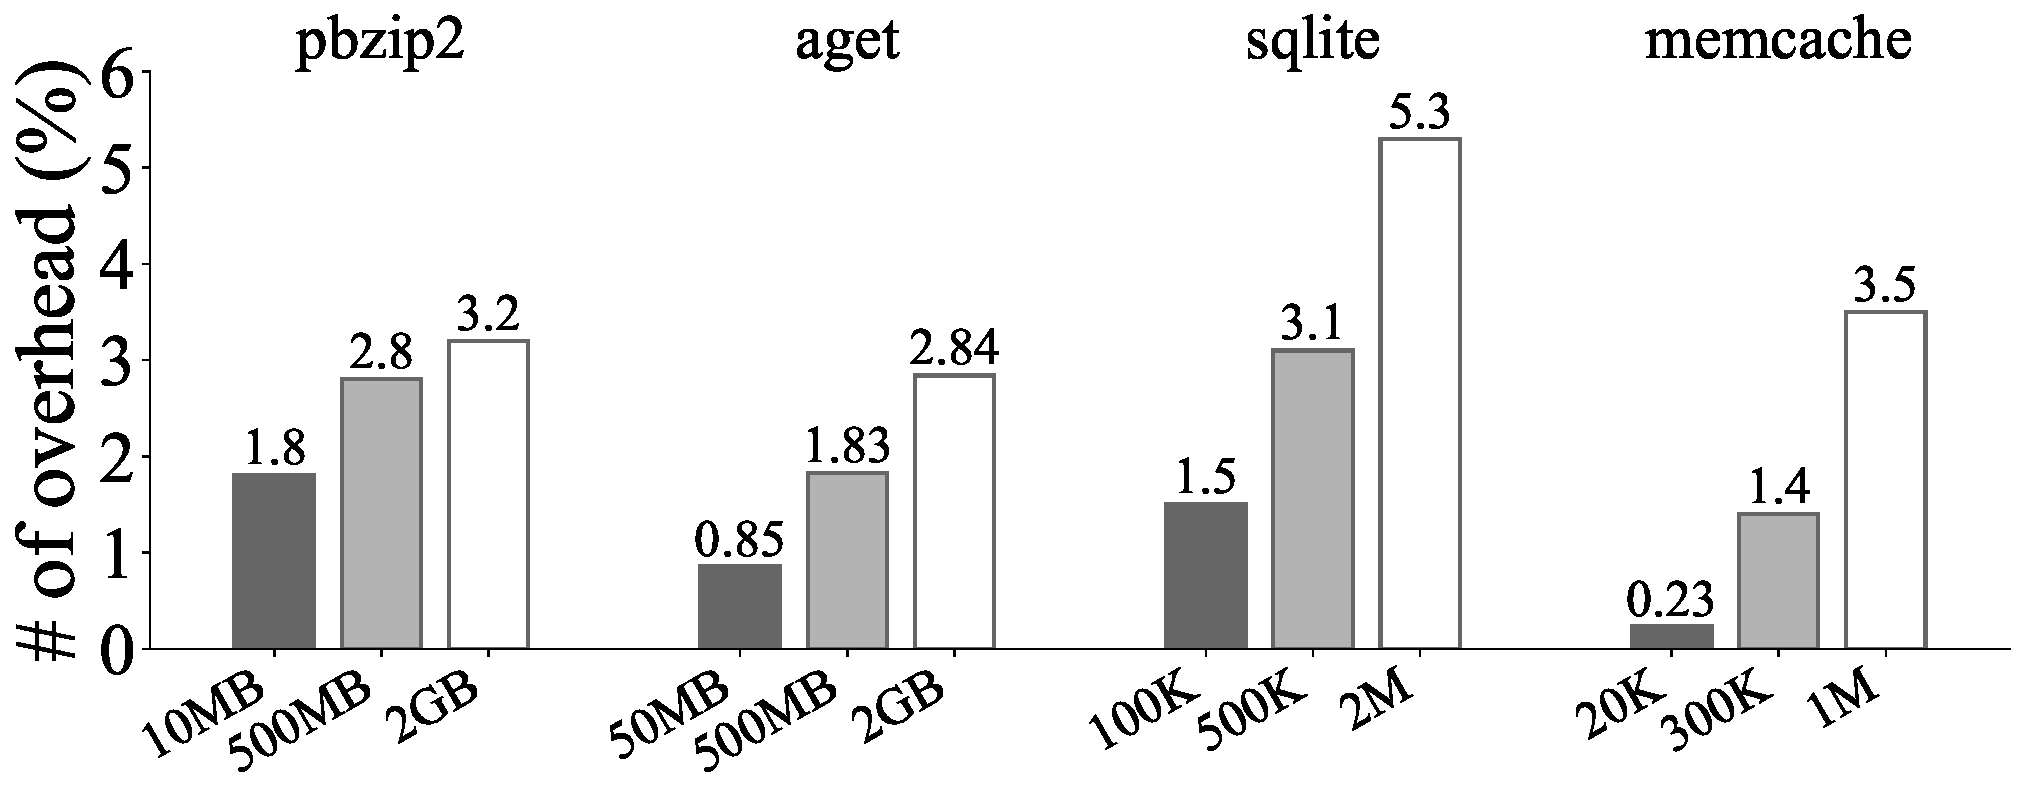
\includegraphics[width=0.9\textwidth]{figures/normaloverheadbar.pdf}
    \caption{Performance overhead of 4 real-world programs}
    \label{fig:Performance overhead of Normal Execution}
\end{figure}


We show performance overhead results in Figure \ref{fig:Performance overhead of
    Normal Execution}.
% For ETM tracing only, control flow tracing incurs a runtime
% performance overhead of 0.0071\% on average with no test exceeding 0.1\%
% overhead across all programs. 
Overall, the average performance overhead of all tests is 2.3\%, and the highest
overhead is 5.3\% for \texttt{SQLite} when writing $2,000,000$ values. The
performance overhead has a slight improvement when test stress increases in all
four programs. We believe it is caused by \TheName because there are many I/O
operations and a large number of \syscall{}s.
%cause more overhead
%than others.

%compare to REPT LAZY
We compare the runtime performance overhead of real-world programs with the
state-of-the-art systems \cite{cui2018rept, kasikci_lazy_2017}. The results show
that our overhead is slightly higher, mainly caused by the
\TheName. Nevertheless, \TheName still incurs a low runtime performance overhead
(2.3\% on average). We conclude this overhead is acceptable and still suitable for
practical deployment.

\subsubsection{Trade-offs Between Performance and Accuracy} \label{space-consumption}

% Since we collect a lot of data at runtime, we need to consider its consumption
% on space illustrate our trade-offs for \Recordingstage.

We design two versions of syscall capturing to record \textit{RC-Type}
\syscall{}s: saving the whole content or truncating to the beginning 256 bytes
. We test the time and space consumption of both
versions by a program that continuously reads a 2 GB text file to simulate a
highly concurrent environment on the server. The experimental results shown in
Table \ref{space_consumption} demonstrate that saving the entire content imposes
a significant overhead (12.5\%). In addition, an estimate for 24 hours of
continuous recording generates nearly 1 TB files, which indicates that saving
the entire content is also impractical for a larger throughput server.
Therefore, we choose to truncate the records of \textit{RC-Type} \syscall{}s to
the beginning 256 bytes.

\begin{table}[]
    % \small
    \caption{Space Consumption for Saving All Content or Truncation}
    \label{space_consumption}
    \centering
    \begin{tabular}{@{}llll@{}}
        \toprule
        \textbf{Type}        & \textbf{Real Time}       & \textbf{File Size} & \textbf{\begin{tabular}[c]{@{}l@{}}Estimated \\ 24-hour File Size\end{tabular}} \\ \midrule
        \textbf{Baseline}    & 2 min 50.3 s             & -                  & -                                  \\
        \textbf{All Content} & 3 min 11.552 s (+12.5\%) & 2.0 GB             & 902.1 GB                           \\
        \textbf{Truncation}  & 2 min 57.675 s (+4.33\%) & 120 MB             & 52 GB                              \\ \bottomrule
    \end{tabular}
\end{table}


\subsection{Universality} \label{subsec:eva-Generality}

In this section, we shows \TheName is a universal tool for almost all Linux devices. \TheName is basically a kernel module that does not need any dependency. All functions of \TheName are implemented in Linux kenrel, which indicates that \TheName is architecture-independent.

I also have verified on different platforms beyond ARM juno board. The specifications of these platforms are as follows.
\begin{itemize}
    \item  \textbf{ARM}: Raspberry Pi 3B, Debian GNU/Linux 10 with Linux 5.10.11-v8+.
    \item \textbf{x86}: Intel Core i5-10500, Ubuntu 18.04.5 LTS with 4.15.0-142-generic.
    \item \textbf{RISC-V}: Qemu 5.2.0 RISC-V virt, Linux 5.11.0.
\end{itemize}

Although \TheName currently does not support all features (e.g., recording for return address) on devices of other architectures, the core part of \TheName, i.e., collecting information and saving to file, works fine. Besides, there are some recent work to make extensions based on \TheName on RISC-V \cite{gdjs2_gdjs2mysisdig_2021}, which also indicates the universality of \TheName.